\documentclass{article}
\usepackage[utf8]{inputenc}


\title{Tarefa 4}
\author{Gabriel Martins Spínola}
\date{\today}


\usepackage{graphicx}
\usepackage{listings}
\usepackage{minted}
\usepackage{hyperref}
\usepackage{amsmath,xparse}

\begin{document}
\begin{titlepage} %iniciando a "capa"
\begin{center} %centralizar o texto abaixo
{\large Universidade Federal do Rio Grande do Norte}\\[0.2cm] %0,2cm é a distância entre o texto dessa linha e o texto da próxima
{\large Instituto Metrópole Digital}\\[0.2cm] % o comando \\ "manda" o texto ir para próxima linha
{\large Bacharelado em Tecnologia da Informação}\\[0.2cm]
{\large Cálculo Numerico para Ciência da Computação}\\[5.0cm]
{\bf \huge Relatório Tarefa 6}\\[5.0cm] % o comando \bf deixa o texto entre chaves em negrito. O comando \huge deixa o texto enorme
\end{center} %término do comando centralizar
{\large Discente: Gabriel Martins Spínola}\\[0.7cm] % o comando \large deixa o texto grande
{\large Docente: Dr. Rafael Beserra Gomes}\\[3.2cm]
\begin{center}
{\large Natal, RN}\\[0.2cm]
{\large 2020}
\end{center}
\end{titlepage} %término da "capa"


\section*{Introdução}
\hspace{0.5cm}Tarefa realizada para a disciplina Cálculo Numérico para Ciência da Computação. Essa, tratou do tema regressão linear e regressão polinomial, onde procuramos calcular funções que aproximem uma certa quantidade de pontos.

\section*{Questão 1}
    \subsection*{A)}\hspace{0.5cm}Para calcular uma função linear dos 1000 pontos dados precisamos fazer uma regressão linear, para isso, foi feito o código a seguir:
    \inputminted[]{python}{questao1.py}
    
    Esse, calcula os valores que serão utilizados no sistema linear para encontrar os valores dos coeficientes da reta ao qual procuramos.
    
    Para calcular esse sistema foi utilizado o algoritmo que foi criado anteriormente em outra tarefa desta disciplina, o algoritmo de eliminação de Gauss. Retornando assim os valores aproximados de $a_0$ e $a_1$, que são, respectivamente -60.066083327 e 70.3336844377. Portanto a função que representa bem a relação entre peso e altura é: y = -60.066083327 + 70.3336844377x
    
    \subsection*{B)}Plotando a função encontrada acima e os pontos que foram dados temos a imagem a seguir:\\
    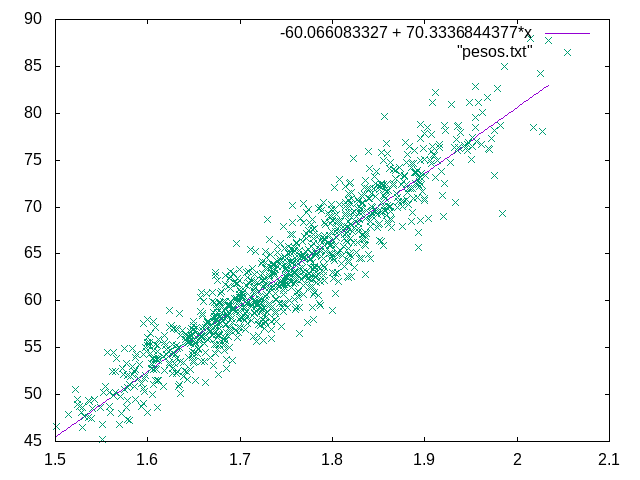
\includegraphics[scale = 0.85]{relacao.png}\\
    
    \subsection*{C)}
    \hspace{0.5cm}Já temos a função que representa bem a relação, portanto, para estimar o peso dessa pessoa, precisamos apenas calcular o valor de y para x = 2,10, portanto, temos que\\
    y = -60.066083327 + 70.3336844377x\\
    y = -60.066083327 + 70.3336844377*(2.10)\\
    y = 87.634654\\
    
    Portando, o peso estimado para uma pessoa de 2m10cm é aproximadamente 87.6Kg
    
\section*{Questão 2}
    \subsection*{A)}\hspace{0.5cm}Para calcular uma função não linear para os pontos dos barcos, vamos calcular um polinomio de grau 2, para isso iremos utilizar o método da regressão polinomial. Para calcular esses pontos, foi feito o código a seguir, que calcula o valor dos somátorios que precisamos:
    \inputminted[]{python}{questao2.py}
    Logo, para calcularmos os coeficientes do polinomio de grau 2 precisamos resolver o sistema linear:\\
    $\begin{bmatrix}
        \Sigma X_i^0 & \Sigma X_i^1 & \Sigma X_i^2\\
        \Sigma X_i^1 & \Sigma X_i^2 & \Sigma X_i^3\\
        \Sigma X_i^2 & \Sigma X_i^3 & \Sigma X_i^4
    \end{bmatrix}$
    $\begin{bmatrix}
        a_0\\
        a_1\\
        a_2\\
    \end{bmatrix}$
    = $\begin{bmatrix}
        \Sigma Y_i\\
        \Sigma Y_iX_i\\
        \Sigma Y_iX_i ^2\\
    \end{bmatrix}$\\
    com os somatórios indo de 1 até 40.
    
    Logo, \\
    $\begin{bmatrix}
        40 & 367.688421059 & 3388.2590212\\
        367.688421059 & 3388.2590212 & 3388.2590212\\
        3388.2590212 & 31299.9556398 & 289849.162995
    \end{bmatrix}$
    $\begin{bmatrix}
        a_0\\
        a_1\\
        a_2\\
    \end{bmatrix}$
    = $\begin{bmatrix}
        233.095081737\\
        2102.5650367\\
        19012.4988953\\
    \end{bmatrix}$\\
    Colocando novamente essa matriz no algoritmo de eliminação de Gauss temos, aproximadamente, que:
    $a_0 = 376.0266354806$, $a_1 = -75.885348890723$, $a_2 = 3.8645787396191$\\
    Portanto, a função não linear que representa bem os pontos dados é a função:\\
    $P_2(x) = a_0 + a_1x + a_2x^2$\\
$P_2(x) = 376.0266354806 -75.885348890723x + 3.8645787396191x^2$  

    \subsection*{B)}A seguir o gráfico obtido com a função e os pontos coletados:\\
    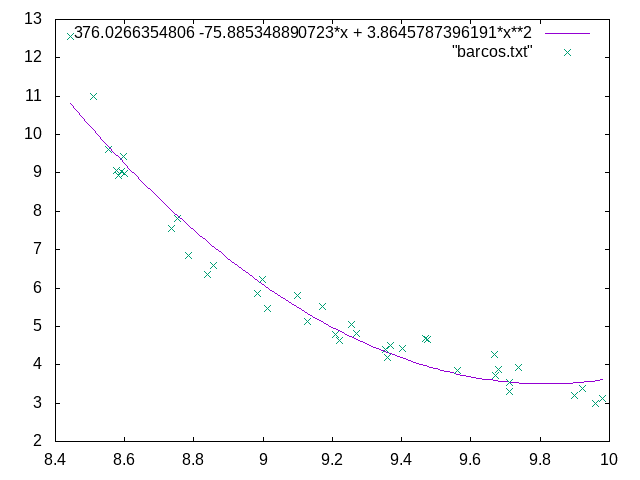
\includegraphics[scale=0.8]{barcos.png}
    
    \subsection*{C)}\hspace{0.5cm}Para estimar o tempo de percuso a 11km/h basta substituir no polinomio:\\
    $P_2(11) = 376.0266354806 -75.885348890723*11 + 3.8645787396191*11^2 = 8.9018251765581$
    
    Portanto, levará 8h9min aproximadamente a uma velocidade de 11km/h
    
    
    \subsection*{D)}\hspace{0.5cm}Sabemos que o barco leva 8h9min para percorrer o rio indo e voltando, a uma velocidade de 11km por hora, portanto, 8.9 * 11 = 97.9km, porém esse é o comprimento do percurso de ida e volta, logo, para sabermos o comprimento do rio basta dividir por 2, portanto, o comprimento do rio é 97.9/2 = 48.95 km
    
    
\section*{Conclusão}
\hspace{0.5cm}A tarefa feita teve por finalidade aprender e utilizar métodos que dados varios pontos, podemos representar esses pontos por meio do comportamento de uma função que será bem próximo em relação ao comportamento dos pontos no gráfico. para isso vimos os métodos da regressão linear, onde procuramos fazer a relação com uma função que representa uma reta, e da regressão polinomial que podemos fazer a relação com funções não lineares.
\end{document}
